\chapter{Design and Implementation}
\label{chap:implementation}
Figure \ref{fig:three-tier-architecture} gives an overview of the three-tier architecture of the jSCAPE system, the relationships between each of the components, and some of the tasks that they perform. The student view is implemented as a JavaFX applet embedded into the web browser. It communicates with a custom written Java application server using a custom built communication protocol. Finally, the application server also connects to a PostgreSQL database, to perform the standard read and write operations. \newline

The admin tool isn't shown in the diagram, but it connects directly to the database for result analysis and exercise bank management. INCLUDE ADMIN TOOL IN DIAGRAM + exercise generator + results analyzer, remove generate exercises from server.

\begin{figure}[H]
\centering
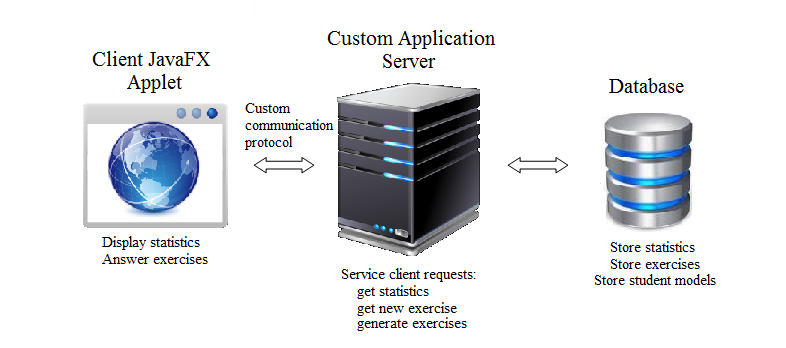
\includegraphics[width=\textwidth,height=\textheight,keepaspectratio]{three-tier-architecture}
\caption{Three tier architecture of the jSCAPE system.}
\label{fig:three-tier-architecture}
\end{figure}

In the rest of this chapter we justify our design choices and discuss the implementation of the various components and features of the jSCAPE system.

\section{Design choices and technology}
Most software in the area of computer based education is web-based, as demonstrated by the review of related work in chapter \ref{chap:related-work}. We decided to follow this trend, as it makes deployment easier, and because students are usually quite familiar with web browsers. There are multiple technologies which can be used to develop a web application. Some of these are HTML5, CSS, Javascript, Flash, and Java applets.\newline

We decided to take the approach of Java applets because we have had a lot of experience with developing large scale programs in this language. In addition, Java applets better encapsulate the functionality into one place, instead of requiring the user to click links on a website to access a feature. Finally, developing jSCAPE as an applet allows it to run in Java web start mode or as a stand alone desktop application, thanks to the Java deployment framework. \newline

However, regular Java applets use the Swing library for GUIs, and as a result, the interface doesn't end up being user-friendly or visually appealing. This is certainly a problem, because although the application can present powerful and useful features, students will only use it if the interface is intuitive and aesthetically pleasing\cite{Interface-study}. \newline

This realisation led us to researching libraries which could improve the interfaces of Java applets, and discovering JavaFX. JavaFX is intended as a replacement for the Swing GUI library, and is designed to provide a lightweight, hardware-accelerated Java UI platform for creating rich internet applications\cite{JavaFX}. The JavaFX library includes a powerful and visually appealing statistics package, with support for pie charts, bar charts, line charts, scatter charts, tables, etc... which was more than enough to implement the statistics tracking and displaying component of jSCAPE. In addition, this would allow us to easily add more displayable statistics in the future (section \ref{sec:future-work}), if required. \newline

JavaFX also provides the functionality of embedding a \textsf{WebView}, a browser component which supports HTML5, CSS and Javascript, into the applet. We found that this could be an interesting feature to use for developing exercises with variety and interactivity, For instance, this component is used in the Binary Tree exercises to display the binary trees (section BINARY TREE EXERCISES). \newline

Server technlogies and design choices, why custom built?\newline

Database technology and design choice. Throughout this chapter, we show how the database is used, which tables are maintained, etc...

\section{Server and client-server communication}
The server is responsible for servicing all client requests, for instance, requesting peformance statistics or requesting a new exercise. It is custom built, multithreaded and written in pure Java, using Sockets and Object input/output streams.
The basic server class and the mechanism to communicate with clients accounts for approximately 300 lines of code. \newline

\lstinputlisting[caption={Serializable message object used for client-server communication.}, label={lst:message.java}]{\listings/message.java}
The code in \ref{lst:message.java} shows the basic unit that travels between the client and the server, and vice-versa. A message consists of a message code, used to determine its structure, and a payload of request parameters, in the form of an \textsf{ArrayList$<$String$>$}.\newline

\lstinputlisting[caption={Message request codes.}, label={lst:message_codes.java}]{\listings/message_codes.java}

The existing message request codes are shown in \ref{lst:message_codes.java}. The server uses these to determine what the client has requested, how the request message is formatted and which actions to perform to service the request. \newline

\lstinputlisting[caption={An example client request.}, label={lst:example_service.java}]{\listings/example_service.java}

The code snippet in \ref{lst:example_service.java} gives an example of how the client can construct a request. In this particular example the client is requesting the statistical data about the student's performance. On line 1, a \textsf{Service} is created. A \textsf{Service} is a task that can be performed over and over again by calling the \textsf{restart()} method, like on line 12. Lines 2 to 10 determine what the service should do when it is started. Lines 4 and 5 add the student's login name as a request parameter. On lines 6 and 7, the message is constructed with the appropriate message code, and the request parameters. On line 9, the message is sent to the server, and the reply from the server is stored in the \textsf{Service}, for the client to use later on.\newline

In addition to communicating with the client, the server also communicates with the PostgreSQL database. This is to retrieve the data requested by the client, and to update the state of the system as the student answers exercises, for instance. Therefore, a database module was created with methods to perform the necessary functions. \newline

\lstinputlisting[caption={An example database retrieval method.}, label={lst:example_database_method.java}]{\listings/example_database_method.java}

In figure \ref{lst:example_database_method.java} we give an example of a database retrieval method. All methods which read from the database return a \textsf{ArrayList$<$String$>$}, so that this can be immediately put in the reply message from the server to the client. In this particular example, the method retrieves performance statistics for the student identified by \textsf{loginName}. Line 6 creates the data structure to hold the information which will be read from the database. Lines 8 to 18 create the query, and send it to the database to be executed. In lines 20 to 24, the result of the query is added to the data structure. Finally, on line 27, all this information is returned to the server, which can now encapsulate this in a reply message, and send that to the client. \newline

This database module is also used by the jSCAPE admin tool to analyze results and manage the exercise bank. The module comprises of 8 classes, one for each database table, and accounts for approximately 1500 lines of code.
\section{Exercises}
talk about Beanshell for ex gen

\subsection{Implementing exercise selection algorithms}

\subsubsection{Random selection}
Random selection

\subsubsection{Selecting based on the difficulty category}

\begin{figure}[H]
\centering
\begin{tikzpicture}[>=stealth',shorten >=1pt,auto,node distance=3cm]
  \node[initial,state] (A1)      {$A1$};
  \node[state]         (A2) [right of=A1]  {$A2$};
  \node[state]         (A3) [right of=A2] {$A3$};
  \node[state]         (B1) [below of=A3] {$B1$};
  \node[state]         (B2) [left of=B1] {$B2$};
  \node[state]         (B3) [left of=B2] {$B3$};
  \node[state]         (C1) [below of=B3] {$C1$};
  \node[state]         (C2) [right of=C1] {$C2$};
  \node[state]         (C3) [right of=C2] {$C3$};


  \path[->] (A1)  edge [loop above] node {wrong} (A1)
             edge [bend left] node {correct} (A2)
        (A2) edge [bend left]  node {wrong} (A1)
             edge [bend left] node {correct} (A3)
        (A3) edge [bend left]  node {wrong} (A2)
             edge [bend left] node {correct} (B1)
        (B1) edge [bend left]  node {wrong} (A3)
             edge [bend left] node {correct} (B2)
        (B2) edge [bend left]  node {wrong} (B1)
             edge [bend left] node {correct} (B3)
        (B3) edge [bend left] node {wrong} (B2)
             edge [bend left] node {correct} (C1)
        (C1) edge [bend left] node {wrong} (B3)
             edge [bend left] node {correct} (C2)
        (C2) edge [bend left] node {wrong} (C1)
             edge [bend left] node {correct} (C3)
        (C3) edge [loop above] node {correct} (C3)
             edge [bend left] node {wrong} (C2);             
\end{tikzpicture}
\caption{State machine of adaptive difficulty categories.}
\label{state-machine}
\end{figure}

Figure \ref{state-machine} shows the state machine implemented by this exercise selection algorithm.

\subsubsection{Selecting using Item Response Theory}

\lstinputlisting[caption={Item information algorithm.}]{\listings/item_information.java}

\lstinputlisting[caption={Item response function algorithm.}]{\listings/item_response_function.java}

\section{Collecting statistical data}
\newpage

Implemented as a JavaFx applet. but it is still possible to run the program with Java web start or as a stand alone desktop application thanks to the Java deployment framework.\newline

Talk about design choices such as only multiple choices, no exercises asking to write code, writing custom server, etc...\newline

Mention three tier architecture\newline

implemented as a JavaFx applet\newline
javafx also good because provides better possibilities for UI instead of the normal Swing look and feel which looks quite old and horrible in our opinion.\newline
javafx provides useful statistics package....pie charts, graphs, tables...\newline

list tools+technology and evaluate advantages/disadvantages\newline

java programming exercises, binary trees and code exercises to show the capabilities of the system, that it can handle multiple types of exercises.\newline

server implementation, message codes, objectin/out streams, serverthread, show example array payload method to transfer stuff between client and server\newline

showing feedback immediately after the exercise....cite source, shown to be most effective way of learning\newline

piece of code + exercise involving the behaviour of the code have been found efficient (lister 2001) as far as student's assessment on their ability to read and understand the code's semantics. (NOT MY OWN WORDS) Lister, R. (2001). Objectives and objective assessment in CS1. ACM SIGCSE Bulletin, Vol. 33, No. 1, pp. 292-296. \newline

CAT development, we refer back to the five components of a CAT...what item selection algorithm we use, what scoring procedure, no termination criterion, entry point is average knowledge distribution initially and attempts at a calibrated item pool, currently with teacher providing the parameters since obtaining a high quality calibrated item pool isn't something I can do.